
Plan approximatif de cette partie :

\begin{enumerate}[label=\Roman* --- ] \bfseries
	
	\item Prérequis \\
	{\normalfont\itshape Dans notre cas, tout s'écrit très simplement donc pas besoin de sortir tout l'arsenal de géo diff}
	\begin{enumerate}[label=\arabic{enumi}.\arabic* --- ]
		
		\item Espace projectif complexe
		\begin{itemize}%[label=\arabic{enumi}.2.\arabic* --- ]
			
			\item Construction de $\PC{n-1}$ 
			\begin{itemize} \normalfont
				
				\item Définition comme espace quotient $\S{2n-1}/\U{1}$
				
				\item $\PC{n}$ vue comme variété différentielle complexe (voir annexe pour détails)
				
				\item \thoughts{lien avec la projection $\x \longmapsto \x\x^\dagger$ utilisé en physique}
				
			\end{itemize}
			
			\item Métrique de Fubini-Study 
			\begin{itemize} \normalfont
				
				\item Métrique induite par la projection
				
				\item expression de la métrique
				
				\item expression en coordonnée local
				
			\end{itemize}
			
		\end{itemize}
		
		\item Fibré principaux
		\begin{itemize}%[label=\arabic{enumi}.1.\arabic* --- ]
			
			\item Fondamentaux
			\begin{itemize} \normalfont
				
				\item Définitions de base
				
				\item Section local (canonique)
				
				\item changement de carte
				
			\end{itemize}
			
			\item Espaces horizontaux et connexion
			\begin{itemize} \normalfont
				
				\item Espace verticaux
				
				\item connexion comme ensemble d'espace horizontaux
				
				\item 1-forme de connexion
				
				\item notre choix de connexion (induite par le produit hermitien)
			\end{itemize}
			
		\end{itemize}
		
	\end{enumerate}
	
	\item Interprétation géométrique des trois phases
	\begin{enumerate}[label=\arabic{enumi}.\arabic* --- ]
		
		\item Cas des signaux ``pseudo-cyclique'' (cyclique à phase près)
 		\begin{itemize} \normalfont
			
			\item Le dessin de Bohm :
			
			\item phase dyn =  signal - horizontal lift
			
			\item phase geo = horizontal lift - cyclique lift (<- indé du signal !)
			
			\item phase tot = cumul des deux
		\end{itemize}
		
		\item La phase géo dans l'espace projectif
		\begin{itemize} \normalfont
			
			\item Géodésique de $\PC{n}$ et généralisation du cas pseudo-cyclique
			
			\item Remarque de Mukunda : phase géo est une 2-forme vs phase dyn est une 1-forme
		
			\item Bonnet-Gauss  \& Stokes : phase géo comme calcul d'air
	
			
			\item \thoughts{Comme partie imaginaire de la métrique \textit{(+ lien avec Fisher)}}
		
		\end{itemize}
	\end{enumerate}
\end{enumerate}
\skipl
\\
\textbf{Annexes}
\begin{enumerate}[label=\Alph* --- ] \bfseries
	
	%\item Forme différentielles \textit{(nécessaire ?)}
	
	\item Algèbre et groupe de Lie
	\begin{itemize}\normalfont
		
		\item def : groupe de Lie $G$
		
		\item def : Algèbre de Lie $\mathfrak{g}$ associée à $G$
		
		\item $\mathfrak{g}$ vu comme tangent $\tg[e]{G}$
		
		\item Cas particulier : $G=\U{1}$
		
	\end{itemize}
	
	\item Variétés différentielles complexe 
	\begin{itemize} \normalfont
		
		\item Complexification de TM
		
		\item L'intérêt de faire ça : proprement définir $\partial/\partial\bar{z}$
		
		\item Exemple : écriture de forme de Kahler de Fubini-Study
		
	\end{itemize}
\end{enumerate}

\newpage


\thoughts{A reprendre, comme toutes les intros} Pour étudier la phase géométrique d'un signal $\psi$, il nous faut projeter $\psi$ sur $\PC{n}$, et ceux, tout en gardant une trace de sa phase puisque c'est le lien entre les deux qui nous intéresse. Il nous faut donc envoyer $\psi$ dans le produit :
\[\U{1}\times \PC{n}\qquad\qquad (\text{ou }\ \C^{n-1*}/\C^*)\]
\\
Garder le lien entre cet espace et celui d'origine mène à se placer dans le cadre avec d'un \emph{variété fibrée} (ou simplement fibré). Plus précisément, comme $\U{1}$ est un groupe de lie, ce sera un \emph{fibré principal} noté $\S{2n+1}\big(\U{1},\PC{n}\big)$.
\\

Comme son nom l'indique, $\S{2n+1}\big(\U{1},\PC{n}\big)$ à une structure de variété différentielle et le lien entre les $\U{1}$ et $\PC{n}$ va se faire par le biais d'une connexion. L'on verra alors que cette connexion est intrinsèquement lié à la phase dynamique du signal, et il sera discuté de la signification de ce résultat.
\\
La phase géométrique, quand à elle, sera liée avec la métrique hermitienne associée aux l'espaces projectifs complexes.
\\
Tout cela va demander quelques prérequis que nous allons voir à présent.
\\



\section{Prérequis mathématique}

\subsection{Variétés différentielles complexes et les espaces projectifs complexes}\label{subsec:PC^n}

Les espaces projectifs complexes se construisent ainsi. On se place dans ${\C^{n+1}}^*=\C^{n+1}\setminus\{0_{\C^{n+1}}\}$ avec la relation d'équivalence, $\forall x,y\in{\C^{n+1}}^*$ :
\[x \sim y\ \Llr\ \exists \lambda\in\C^*\ |\ x=\lambda y\]
\\
L'espace projectif complexe, noté $\PC{n}$, est l'espace quotient :
\[\PC{n} = {\C^{n+1}}^*/\C^* = {\C^{n+1}}^*/\sim\]
\\
En notant $[z]$ la classe de $\PC{n}$ du représentant $z = (z^i)_{0\leq i\leq n}\in{\C^{n+1}}^*$, on définit les ensembles et cartes, $\forall i\in\llbracket0,n\rrbracket$ :
\begin{align}
	U_i &= \Big\{[z]\in\PC{n}\ \big|\ z^i\neq 0\Big\}  &  \phi_i\  :\quad &\begin{aligned}
		U_i\ \ &\lr\quad\ \C^{i}\times \{1\} \times\C^{n-i}\cong \C^{n} \\ [z]\ \ &\lmt\ \frac{1}{z^i}\big(z^0,\cdots, z^i,\cdots, z^n\big)
	\end{aligned}
\end{align}
\\
L'ensemble d'arrivé $\phi_i(U_i)$ est de dimension $n$ et s'assimile à $\C^{n}$ mais, par souci de comodité, on restera dans $\C^{n+1}$. Cela permet  d'écrire plus simplement les formules de changement de carte en évitant de devoir enlever et rajouter des coefficients :
\[ \forall [z]\in U_i\cap U_j\quad (\ie~z^{i,j}\neq 0) ,\qquad \phi_i \circ {\phi_j}^{-1}(z) = \frac{z^j}{z^i}z\]

Les $(U_i,\phi_i)$ forment ainsi un atlas holomorphe sur l'espace projectif complexe, faisant de $\PC{n}$ une variété complexe de dimension $\dim[\C] = n$ (voir annexe \ref{ann:variet_complexe} pour plus de détail).


\begin{proposition}
	$\PC{n}$ admet une métrique hermitienne induite par la métrique de $\S{2n+1}$, elle même induite du produit scalaire sur $\R^{2n+1}$. Elle est appelé \emph{métrique de Fubini-Study} et est donnée par le formule :
	\[\]
\end{proposition}
\skipl



\subsection{Variété fibrée principale et connexion} \label{subsec:VFP}

Pour le dire simplement, les \emph{variétés fibrés} sont des variétés qui ressemble localement à des espaces produits. 
Le ruban de Modiüs en est un exemple typique : il ne peut pas s'écrire comme le produit d'un cercle avec un segment $\S{1}\times [0,1]$ à cause de la façon dont il est construit. Mais localement, il est tout à fait comparable (\ie~difféomorphe) à un tel produit (\cf~\cref{fig:ruban2modius}).
\begin{figure}[h]
	
\includegraphics[width=0.45\textwidth]{fig/placeholder}
	%\begin{tikzpicture}[scale=0.8]
	%\draw[opacity=0.1] (-4.5,-4.5) grid (12.5,4.5);
	
	
%%%%     MOBIUS     %%%%

	%main points
	\coordinate (s1-) at ($(90+0-30:4) + (0,-1)$);
	\coordinate (s1+) at ($(90+0+30:4) + (0,-1)$);
	
	\coordinate (s2+) at ($(90+120-30:4) + (0,-1)$);
	\coordinate (s2-) at ($(90-120+30:4) + (0,-1)$);
	
	\coordinate (s3+) at (90+120+30:4);
	\coordinate (s3-) at (90-120-30:4);
	
	%\draw (s1-) -- (s2+) -- (s3-) -- (s1-);
	%\draw (s1+) -- (s3+) -- (s2-) -- (s1+);
	%\draw (s3+) -- (s3-);
	\colorlet{tmpb}{blue!30!};
	\colorlet{tmpr}{red!30!};
	\colorlet{tmpv}{blue!30!red!30!};
	\definecolor{tmpg}{gray}{0.75};
	
	
	% bande droite
	\draw[fill=tmpr] (s1-) .. controls  ($(s1-)+(-60:3)$) and  ($(s3+)+(0:3)$) .. 
		(s3+) -- (s3-) 
		.. controls ($(s3-)+(0:1)$) and ($(s2-)+(-60:1)$) .. 
		(s2-) -- cycle;
		
	% bande haut
	\draw[fill=tmpv] (s1-) .. controls  ($(s1-)+(120:0.5)$) and  ($(s1+)+(60:0.5)$) .. 
		(s1+) -- (s2+) 
		.. controls ($(s2+)+(60:2)$) and ($(s2-)+(120:2)$) .. 
		(s2-) -- cycle;
		
	% bande gauche
	\draw[fill=tmpb] (s1+) .. controls  ($(s1+)+(-120:3)$) and  	($(s3-)+(-180:3)$) .. 
		(s3-) -- (s3+) 
		.. controls ($(s3+)+(-180:1)$) and ($(s2+)+(-120:1)$) .. 
		(s2+) -- cycle;
		
		
	%%%%     CARTE LOCALE     %%%%
	
	% ouvert U_i
	\draw (-1,0.25) -- (-1.5,2.67) node[midway, above right]{$U_i$};
	\draw (1,0.25) -- (1.5,2.67);
	
	% carte
	\draw[fill=tmpg, shift={(6.25,-1.5)}] (0,0) -- (0, 4) node[midway, left]{$G$} -- (3.5,4) -- (3.5,0) -- cycle node[midway, below]{$\pi(U_i)$};
	
	% fleche vers la carte
	\draw[-Stealth, thick] (0,2.5) ..
	controls ($(0,2.5) + (30:2)$)  and ($(7, 2) + (180-30:2)$) .. (7, 2) node[midway, above]{$h_i$};
	
\end{tikzpicture}
	\caption[Ruban de Mobius comme variété fibrée]{Représentation du ruban de Modius en tant que fibré. Les notations sont reprise de la \cref{def:VFP}.}
	\label{fig:ruban2modius}
\end{figure}
\skipl

Il existe toutes sorte de variétés fibrées dès lors qu'elles sont munies de structure remarquable. Celles qui vont nous intéresser sont celle dites principales\footnote{\itshape
	Bien que ce ne sera pas précisé, il sera toujours sous-entendu que les différentes variétés et cartes doivent avoir les mêmes niveaux de régularités pour que le tout reste cohérent.} :
\\
\begin{definition}[Variété fibrée principale] \label{def:VFP}
	Une \emph{variété fibrée principale}(VFP), ou \emph{fibré principal} est constituée de deux variétés différentielles $P$ et $B$ telles que :
	\begin{itemize}
		\item Il existe un groupe de Lie $G$ opérant à droite (ou à gauche) sur $P$ via l'application différentiable :
		\begin{equation} \label{eq:VFP_action}
			R\ :\ \begin{aligned}P\times G\ &\lr\quad\ \ P \\ (p,g)\ \ &\lmt\ R_g(p)\defeq p\cdot g = pg
			\end{aligned}
		\end{equation}
		
		\item Il existe une surjection différentiable $\ \pi:P\lr B\ $ telle que :
		\begin{equation} \label{eq:VFP_fibres}
			\forall p\in P,\quad \pi^{-1}\big(\pi(p)\big)=pG
		\end{equation}
		
		\item $P$ est munie d'un ensemble de paire $(U_i, h_i)$ tel que les $U_i$ forment un recouvrement de $B$ et tel que les $h_i : G\times U_i\lr \pi^{-1}(U_i)\subset P$ soient des difféomorphismes vérifiant :
		\begin{align*} \label{eq:VFP_atlas}
			\forall a,b\in G,\ \forall x\in B,\qquad h_i(ab,x) = h_i(a,x) \cdot b\qquad \text{et} \qquad \pi\circ h_i(a,x) = x
		\end{align*}
	\end{itemize}
	
	\begin{adjustbox}{valign=C,raise=1cm, minipage={1.1\linewidth}}
		\begin{wrapfigure}{r}{0.35\textwidth}
			\begin{tikzcd}[column sep=large]
				G\times U_i \arrow[d, "\pr{2}" left]  \arrow[r, "h" above]  & \pi^{-1}(U_i) \subset P \arrow[ld, "\pi" below right] \\
				U_i
			\end{tikzcd}
			%\caption{Digramme sûrement osef des jeux de projections entre $P$ et les cartes locales}
			\label{diagram_commu_VFP}
		\end{wrapfigure} 
		\vspace*{-0.5cm} % This is a fudge to align the top of the theorem environment with the image
		\skipl\par 
		La variété $B$ est appelé la \emph{base} de la VFP, $G$ son \emph{groupe structural} et $pG$ la \emph{fibre de $P$ passant par} $p$ et \emph{au dessus de} $\pi(p)\in B$. Le tout est notée $P(R, G, \pi, B)$ ou plus simplement $P(G,B)$.
		
		Les fibres $pG$ sont toutes difféomorphes à $G$ et $B$ est difféomorphe à $P/G$. Le diagramme commutatif ci-contre résume la situation ($\text{pr}_i$ est la projection canonique sur la $i-$ème composante).
	\end{adjustbox}
\end{definition}
\skipl 


L'ensemble $\big\{(U_i\times G, h_i)\big\}_i$ est l'équivalent d'un atlas pour les variétés différentielles classiques mais adapter pour tenir compte de la structure fibré de $P$ et de l'action de $G$. Explicité les changements de cartes dans $P$, ce fait comme suit.
\\
D'abord, $P$ étant localement difféomorphe à un produit $G\times U_i$, on peut y tracer des graphes appelés \emph{sections locales}, comme sur la \Cref{fig:section_local} \thoughts{ci-dessous}. Formellement, une section locale au dessus  de $U_i \subset B$ est une application $\sigma : U_i \lr P$ vérifiant :
\[\pi\circ \sigma = id_{{\displaystyle |}U_i}\]
\begin{figure}[H]
	\begin{floatrow}
		\ffigbox{\caption[Représentation d'une section local]
			{Représentation d'une section local $\sigma$ au dessus de $U_i\subset\R^2$. Comme $P$ n'est pas un produit à proprement parler, $\sigma$ est représenté dans $G\times U_i$ à travers $h_i$.}
			\label{fig:section_local}}{
			%
\includegraphics[width=0.45\textwidth]{fig/placeholder}
			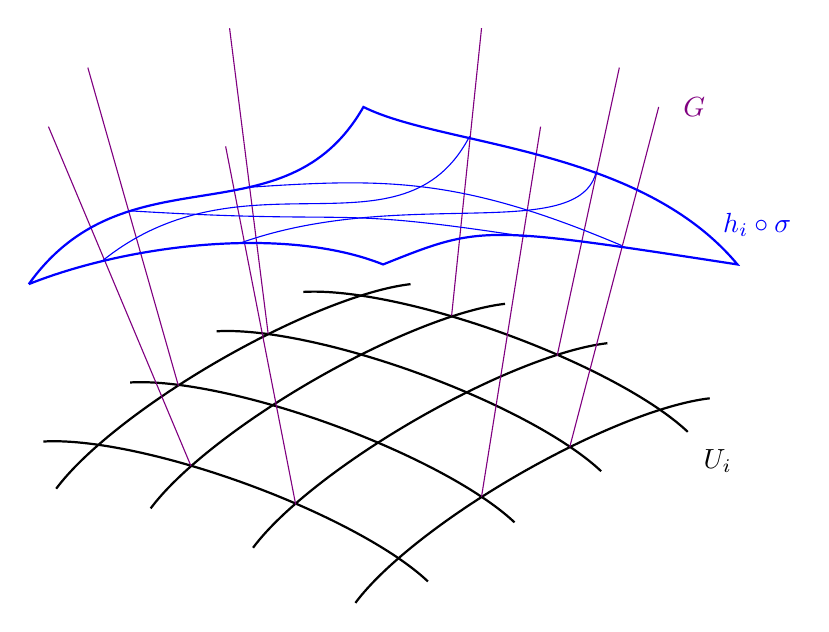
\begin{tikzpicture}%[scale=0.9]
	%\draw[opacity=0.1] (-4.5,-4.5) grid (4.5,4.5);

	%\draw (-1,-4)  .. controls (0,-2.5) and (1.5,-1.75) ..  (4,-2);

% BASE

	% gauche
	\draw[thick, xshift=1.3cm, yshift=-3.2cm, rotate=30]
		(3,0) arc [start angle=30, end angle =150, radius = 3, y radius = 0.75];
		
	\draw[thick, xshift=0cm, yshift=-2.5cm, rotate=30]
		(3,0) arc [start angle=30, end angle =150, radius = 3, y radius = 0.75];
		
	\draw[thick, xshift=-1.3cm, yshift=-2cm, rotate=30]
		(3,0) arc [start angle=30, end angle =150, radius = 3, y radius = 0.75];
		
	\draw[thick, xshift=-2.5cm, yshift=-1.75cm, rotate=30]
		(3,0) arc [start angle=30, end angle =150, radius = 3, y radius = 0.75];
		
	% droite
	\draw[thick, xshift=-2.5cm, yshift=-3cm, rotate=-20]
		(3,0) arc [start angle=30, end angle =150, radius = 3, y radius = 0.75];
	
	\draw[thick, xshift=-1.4cm, yshift=-2.25cm, rotate=-20]
		(3,0) arc [start angle=30, end angle =150, radius = 3, y radius = 0.75];
	
	\draw[thick, xshift=-0.3cm, yshift=-1.6cm, rotate=-20]
		(3,0) arc [start angle=30, end angle =150, radius = 3, y radius = 0.75];
	
	\draw[thick, xshift=0.8cm, yshift=-1.1cm, rotate=-20]
		(3,0) arc [start angle=30, end angle =150, radius = 3, y radius = 0.75];
	
	
% FIBRES

	\draw[violet] (-1.36,-3.05) -- (-2.25,1.5);
	\draw[violet] (1,-2.95) -- (1.75,1.75);
	
	\draw[violet] (-2.69,-2.56) -- (-4.5,1.75);
	\draw[violet] (2.12,-2.32) -- (3.25,2);
	
	\draw[violet] (-2.85,-1.54) -- (-4,2.5);
	\draw[violet] (1.96,-1.16) -- (2.75,2.5);
	
	\draw[violet] (-1.71,-0.88) -- (-2.2,3);
	\draw[violet] (0.62,-0.65) -- (1,3);
	
	
% SECTION

	%frame
	\draw[thick, blue] (-4.75,-0.25) .. controls (-3.5,1.5) and (-1.5,0.25) ..  
		(-0.5,2) .. controls (0.5,1.5) and (3,1.5) ..
		(4.25,0) .. controls (1,0.5) ..
		(-0.25,0) .. controls (-1.5,0.5) and (-3.5,0.25) ..
		(-4.75,-0.25);
		
	% coordo droite
	\draw[blue] (-3.45,0.68) .. controls (-0.5,0.5) and (-1,0.75) .. (1.58,0.35);
	\draw[blue] (-1.95,0.98) .. controls (-0.2,1.1) and (0.75,1.1) .. (2.78,0.24);
	
	%coordo gauche
	\draw[blue] (-3.81,0.05) .. controls (-2,1.5) and (0,0) .. (0.85,1.63);
	\draw[blue] (-2.04,0.28) .. controls (0,1) and (2.25,0.25) .. (2.46,1.19);
	
% NOTATION
	\draw (4,-2.5) node{ $U_i$};
	\draw (3.7,2) node{\color{violet} $G$};
	\draw (4.5,0.5) node{\color{blue} $h_i \circ \sigma$};
	
\end{tikzpicture}}
		
		\ffigbox{\caption[Représentation de la section canonique]
			{Représentation de la section canonique définie par rapport à $G$ avec une seconde section  $\sigma(x) = \sigma_i(x)\cdot g(x)$.% Sont également représentés leur espaces tangents horizontaux respectifs avec la transformation permettant de passer l'un à l'autre.
		}}{
			
\includegraphics[width=0.45\textwidth]{fig/placeholder}
			\label{fig:section_cano}}
	\end{floatrow}
\end{figure}
\noindent
Ensuite, les hypothèses sur $P(G,B)$ sont telles que $G$ agit transitivement et librement (ou sans point fixe) sur $P$. C'est-à-dire que, sur une même fibre, tout point peut être atteint par n'importe quel autre via l'action de $G$ (transitivité) :
\begin{align*}
	\forall x\in B,\quad \forall p,q\in P_x,\ \exists t(p,q)\in G\ |\ p = q\cdot t(p,q) 
\end{align*}
et que la seule façon de laisse les points invariants par cette même action est de passer par l'élément neutre $e$ (libre) :
\begin{align*}
	\forall (p,g)\in P\times G,\quad p = p\cdot g\ \Lr\ g=e
\end{align*}
\\
De la transitivité de $G$, découle le fait que toutes les sections locales $\sigma$ au dessus de $U_i$ peuvent s'écrire à partir d'une même section $\sigma_i$ via la formule :
\[\forall x\in B,\qquad \sigma(x) = \sigma_i(x) \cdot t\big(\sigma_i(x), \sigma(x)\big)\]
Son caractère libre, lui assure l'unicité d'un choix canonique de section $\sigma_i$ sur $U_i$. Elle est donnée par :
\[{h_i}(x,e) = \sigma_i(x)\]
Cela mène à la définition :
\begin{definition}[Fonctions de transitions]
	L'intersection de deux cartes  est noté $U_{ij} = U_i\cap U_j$ et le passage d'une section local canonique est donné par :
	\[\forall x\in U_{ij},\qquad \sigma_j(x) = \sigma_i(x) t\big(\sigma_i(x), \sigma_j(x)\big)\]
	L'élément de $G$, $t(\sigma_i, \sigma_j)$, est alors appelé \emph{fonction de transition} et sera noté $\varphi_{ij}$. Elle fait effectivement la transition entre deux cartes dans le sens où :
	\[\forall (g,x)\in G\times U_{ij},\qquad {h_i}^{-1} \circ h_j(g,x) = \big( \varphi_{ij}(x)g, x \big)\]
\end{definition}
\skipl

Dans la suite, il sera nécessaire de munir $P$ d'une connexion, qui s'introduit comme suit.
\\
Comme $P$ ressemble localement à un produit $G\times U_i$, il est utile de séparer ses espaces tangents $\tg[p]{P}$ comme une somme directe d'espaces tangents respectivement aux fibres et à la base. Conformément aux représentations précédentes (\cref{fig:ruban2modius,fig:section_cano,fig:section_local}), les premiers sont appelées espaces tangents \emph{verticaux}, les seconds \emph{horizontaux} et l'on note :
\[\forall p\in P,\qquad \tg[p]{P} = \vg[p]{P} \oplus \hg[p]{P}\]
\\
Les tangents verticaux $\vg[p]{P}$ se définissent canoniquement par rapport à $\pi$. Pour cela, la \emph{fonction tangente} (ou \emph{dérivée}) \emph{de $\pi$ au point} $p$ est noté $\tg[p]{\pi}$ avec :
\[(\tg[p]{\pi})^i_j = \frac{\partial \pi^i}{\partial x^j}(p) = \partial_j\pi^i(p)\]
\\
Ainsi, $\tg[p]{\pi}$ est à valeur de $\tg[p]{P}$ dans $\tg[\pi(p)]{B}$ et l'espace tangent vertical au point $p$ se défini comme :
\[\vg[p]{P} \defeq \Ker (\tg[p]{\pi}) = \big\{ v\in\tg[p]{P}\ |\ \tg[p]{\pi}(v)=0 \big\}\]
\\ 
Il s'avère que les espaces horizontaux ne peuvent pas être construit de cette façon. Il faut donc faire un choix pour les $\hg[p]{P}$ et c'est ce choix qui est appelé connexion (elle connecte les esapce tangents entre eux).
Ces sous-espaces peuvent être caractérisé par une 1-forme différentiable $\conn$ sur $P$ à valeur dans $\vg[p]{P}$, auquel cas :
\[\forall p\in P,\quad \hg[p]{P} = \Ker(\conn_p)\]
\skipl

Dans le cas des VFP, une connexion doit en plus avoir de bonnes propriétés au regarde de l'action $R$, aboutissant à la définition :
\begin{definition}[Connexion sur VFP] \label{def:connexion2VFP}
	Une \emph{connexion} sur une VFP $P(G,B)$ est la donnée d'un sous-espace tangent, $\hg[p]{P}\subset \tg[p]{P}$, en tout point de $p\in P$ tel que :
	\begin{itemize}
		
		\item $\hg{P}$ dépend différentiellement de $p$ (``dépendre différentiellement'' à un sens précis mais qui ne sera pas utile pour la suite).
		
		\item $\hg[p]{P}$ est supplémentaire à $\vg[p]{P}$ dans $\tg[p]{P}$ :
		\begin{equation}\label{eq:TP=V+H}
			\tg[p]{P} = \vg[p]{P} \oplus \hg[p]{P}
		\end{equation}
		
		\item l'assignation des $\hg[p]{P}$ est invariantes pas l'action de $G$ au sens où :
		\begin{equation}\label{eq:conn_G-inv}
			\forall (p,g)\in P\times G,\quad \hg[R_g(p)]{P} = \tg[p]{R_g} (\hg[p]{P}) = \big\{\tg[p]{R_g}(v)\ |\ v \in \hg[p]{P} \big\}
		\end{equation}
	\end{itemize}
\end{definition}
\skipl

Au delà d'assurer une compatibilité avec la connexion, l'équation \eqref{eq:conn_G-inv} permet de n'avoir à définir la connexion qu'en un seul point de chaque fibre, les autres se déduisant par l'action de $G$. Entre autre, pour tout point de la base $x\in B$, il suffit de la définir en $\sigma_i(x) = h_i(e, x)$ et l'espace horizontale en tout autre point $\ p=h_i(x,g) = \sigma_i(x)\cdot g$ au dessus de $x$ est donné par :
\[\hg[p]{P} = \tg[\sigma_i(x)]{R_g} (\hg[\sigma_i(x)]{P})\]
\\
De même, la 1-forme de connexion n'a besoin d'être définie que sur un point particulier au dessus de chaque fibre. Les espaces verticaux étant tous difféomorphes à l'algèbre de Lie $\mathfrak{g}\cong \tg[e]{G}$ de $G$, c'est sur $\mathfrak{g}$ qu'elle est définie :

\begin{definition}
	La \emph{1-forme de connexion} $\conn$ d'une VFP $P(G,B)$ est définie comme la 1-forme différentiable sur $P$ à valeur dans $\mathfrak{g}$ (\ie~en tout point $p\in P$, $\conn_p$ est valeur de $\tg[p]{P}$ dans $\mathfrak{g}$), telle que :
	\begin{equation} \label{eq:1-form2conn}
		\forall p\in P,\quad \hg[p]{P} \defeq \Ker(\conn_p)
	\end{equation}
	\skipl
	
	En terme de coordonnée local, $\conn$ elle n'a pas besoin d'être définit sur $\ U_i\times G$, mais seulement sur $\ U_i \cong U_i \times \{e\}$. Ainsi, $\conn$ induit une 1-forme sur les cartes $U_i$ par l'image réciproque des sections canonique $\sigma_i$. Elles sont notées $\locconn_i \defeq \sigma_i^*\conn$ et sur le chevauchement $U_{ij}$, elles vérifient :
	\begin{equation}\label{eq:conn_local}
		\locconn_j = {\varphi_{ij}}^{-1} \locconn_i \varphi_{ij} + {\varphi_{ij}}^{-1} \d \varphi_{ij}
	\end{equation}
\end{definition}
\skipl

Si $\locconn_i$ est définie sur les $U_i$, plutôt que $U_i\times G$, c'est encore  grâce à la compatibilité de la connexions avec la l'action de $G$ sur $P$, qui l'information sur $G$ redondante. \thoughts{MEH}. 
\\



\section{Interprétation des trois phases dans ce cadre}

\subsection{HHHHH}

blablabla maintenant on peut recoller les morceaux.
 
Comme $\PC{n}$ est une variété quotient, elle induit naturellement une variété principale :
\begin{proposition}
	La $2n+1$--sphère $\S{2n+1}$, vu comme variété plongée dans $\C^n$ est une VFP de base $\PC{n}$ et de fibre type $\U{1}$. L'action de $\U{1}$ sur $\S{2n+1}$ étant induite par le produit complexe classique et où :
	\begin{itemize}
		\item La fibration $\pi$ est la projection canonique de $\S{2n+1}$ sur $\PC{n}$ :
		\[\pi\ :\ \begin{aligned}\S{2n+1}\ &\lr\ \PC{n} \\ x\quad\ &\lmt\ \ [x]\end{aligned}\]
	
	\item Les cartes locales $h_i$ sont telles que :
	\[\forall z \in \pi^{-1}(U_i),\  {h_i}^{-1}(z) = \big( z_i/|z_i|, [z] \big)\in \U{1} \times \PC{n}\]
	
	\item Tout les représentant $z$ d'un élément de la base $\zeta\in\PC{n}$ sont normé, ainsi, alors tout La section canonique au dessus des $U_i$, $\sigma_i$ elle est définie par :
	\[\]
	
	\end{itemize}
	
	Voir \cite[lemme 2.17]{lafontaine_introduction_2015} pour une démonstration de l'aspect fibré.
\end{proposition}
\subsection{Cas pseudo-cyclique}





%%%% ANNEXES %%%%



\begin{annexe}

\section{Annexe}

\subsection{Connexion induite par une métrique}

Si $P(G,B)$ une VFP munie d'une métrique riemannienne $g$. La connexion induite par $g$ sur $P$ est définie par :
\begin{equation}
	\forall p\in P,\quad \hg[p]{P} = \vg[p]{P}^\perp
\end{equation}
\\
Plus concrètement, $\vg[p]{P}$ est isomorphe à $\mathfrak{g}$ via la transformation :
\[\forall p\in P,\ \forall a\in\mathfrak{g},\quad a^*(p) = \frac{d}{dt} p\cdot \exp(t a)\big|_{t=0} = \frac{d}{dt} p\cdot \exp(t a)\big|_{t=0}\defeq pa\]
\\
Avec, une base $\{\mathfrak{e}_i\}_{1\leq i\leq k}$ de $\mathfrak{g}$ induit un base $\{e_i\}_{1\leq i\leq k} = \{\mathfrak{e}^*_i\}_{1\leq i\leq k}$ sur $\vg[p]{P}$. La métrique $g$ induit alors une connexion de 1-forme :
\[\conn_g(X) = \sum_i g(X, e_i) \mathfrak{e}_i = \sum_i g_{ij}X^j \mathfrak{e}_i\]
\\
et on la projection de $X$ sur $\vg{P}$ est donnée par :
\begin{align*}
	\ver X = \conn(X)^*\quad &\Llr\quad  \ver (X^ie_i) = \sum_i g_{ij}X^j e_i \\
	&\Llr\quad  (\ver X)^i = g_{ij}X^j
\end{align*}


\subsection{Algèbre et groupe de Lie} \label{ann:2Lie}




\subsection{Variété différentielle complexe, tiré de \cite{nakahara_geometry_2003}}

Pour mémoire, une variété différentielle de classe $C^k$ ($k\in\N\cup\{\infty\}$) de dimension $n$ est un espace topologique\footnote{\itshape
	La topologie de $\manu$ doit vérifier des propriétés type séparable, dénombrable à l'infinie, \etc, qui seront toutes admises dans la suite, voir par exemple \cite[chap. 2]{lafontaine_introduction_2015}}
$\manu$ (ou $\manu^n$) munie d'un \emph{atlas} $(\phi_i, U_i)_{i\in I}$, c'est-à-dire un ensemble finie de pair d'ouvert $U_i\subset \manu$ et d'application $\phi_i :U_i\ \lr\ \R^n$ telle que :
\begin{itemize}
	
	\item les $U_i$ forme un recouvrement de la variété :\qquad $\bigcup_{i\in I} \phi_i(U_i) = \manu$
	
	\item les $\phi_i$ sont des homéomorphismes sur leur image $\phi_i(U_i)\subset\R^4$.
	
	\item si l'intersection $U_i \cap U_j$ est non vide, alors ${\phi_j \circ {\phi_i}^{-1}}_{| {\phi_i}^{-1}(U_i\cap U_j)}$ est un $C^k$ difféomorphisme sur son image.
\end{itemize}

$\manu$ sera une \emph{variété différentielle complexe} si elle satisfait les propriétés ci-dessus où $\R^n$ est remplacé par $\C^n$ et où la condition de difféomorphisme est remplacé par la condition d'holomorphisme. 
\\
Une application $f : \C^n\lr \C^n$ étant holomorphe si chacune de ses composantes vérifie l'équation de Cauchy-Riemann :
\[\forall x,y\in\R^n,\ \forall \mu,\qquad \frac{\partial f }{\partial y^\mu}(x+iy) = i \frac{\partial f }{\partial x^\mu}(x+iy)\]
\\
Les fonctions holomorphes étant automatiquement $C^\infty$, les variétés différentielles complexes sont toujours lisse, c'est-à-dire $C^\infty$. Aussi, $\manu$ est dite de dimension complexe $n$ et dimension (réel) $2n$, notés :
\begin{align}\label{eq:manuC-base_cano}
	\dim[\C](\manu) &\defeq n  &  \dim[\R] (\manu) \defeq \dim (\manu) = 2n
\end{align}
\\

Ensuite, pour le dire rapidement, la structure complexe de $\manu$ permet de séparer les espaces tangents en deux sous espaces. Pour ce faire, on commence par noter qu'en tout point $p\in\manu$ de coordonnée $z^\nu=x^\nu+iy^\nu$, l'espace tangent $\tg[p]{\manu}$, vu comme variété réelle, admet une base :
\begin{equation}
	\tg[p]{\manu} = \vec \left\{ \frac{\partial}{\partial x^1}, \cdots, \frac{\partial}{\partial x^n}, \frac{\partial}{\partial y^1}, \cdots,  \frac{\partial}{\partial y^n} \right\}
\end{equation}
\\
Plus tôt que de se basé sur les $x^\mu$ et $y^\mu$ pour séparer les $\tg[p]{\manu}$, on définit sur ces derniers un tenseur $J_p$ de type (1,1) tel que :
\begin{align}
	J_p \frac{\partial}{\partial x^\mu} &= \frac{\partial}{\partial y^\mu}  &  J_p \frac{\partial}{\partial y^\mu} &= -\frac{\partial}{\partial x^\mu}
\end{align}
\\
Ce tenseur est l'équivalent de la multiplication par $\pm i$ et le fait que $\manu$ soit complexe assure qu'il soit défini globalement, \ie~sur $\tg{\manu}$. Il est diagonaliseable dans la base :
\begin{align}\label{eq:manuC-base_holo}
	\partial_\mu = \frac{\partial}{\partial z^\mu} &\defeq \frac{1}{2}\left( \frac{\partial}{\partial x^\mu} - i\frac{\partial}{\partial y^\mu} \right)  
	&  
	\partial_{\bar{\mu}} = \frac{\partial}{\partial \overline{z}^\mu} &\defeq \frac{1}{2}\left( \frac{\partial}{\partial x^\mu} + i\frac{\partial}{\partial y^\mu} \right)
\end{align}
\\
Ainsi en fonction de la base (\eqref{eq:manuC-base_cano} ou \eqref{eq:manuC-base_holo}), $J_p$ va s'écrire :
\begin{align}
	J_p &= \begin{pmatrix}
		\text{\large\ 0\ }\Big. & I_n \\ -I_n & \text{\large\ 0\ }\Big.
	\end{pmatrix}  &
	J_p &= \begin{pmatrix}
		iI_n & \text{\large\ 0\ }\Big. \\ \text{\large\ 0\ }\Big. & -iI_n
	\end{pmatrix} 
\end{align}
\\
Finalement, $\tg{\manu}$ peut être séparé en deux sous-espaces engendré respectivement par les $\partial_\mu$ et $\partial_{\bar{\nu}}$. On parle de vecteur holomorphe et anti-holomorphe et on note :
\begin{align}
	\tg[p]{\manu}^+ &= \Vec\big\{ \partial_\mu\ |\ 1\leq \mu\leq n \big\}  &  \tg[p]{\manu}^- &= \Vec\big\{ \partial_{\bar{\mu}}\ |\ 1\leq \mu\leq n \big\}
\end{align}

\end{annexe}


